\documentclass{article}
\usepackage[T1]{fontenc}
\usepackage{lmodern}
\usepackage{graphicx}
\usepackage{amsmath,amssymb}
\usepackage[a4paper,margin=2cm]{geometry}
\usepackage[absolute,overlay]{textpos}
\setlength{\TPHorizModule}{1mm}
\setlength{\TPVertModule}{1mm}
\usepackage[indonesian]{babel}
\usepackage{hyperref}
\setlength{\emergencystretch}{2em}
% unit: Halaman 4

\begin{document}

% === Halaman 4 (python/native) ===

• Catat bahwa DES adalah sebah standard, sedangkan 

algoritmanya sendiri bernama DEA (Data Encryption 

Algorithm). Kedua nama ini sering dikacaukan.

• DES termasuk ke dalam algoritma kriptografi kunci-

simetri dan tergolong ke dalam cipher blok. 

• DES beroperasi pada ukuran blok plainteks 64 bit. 

• Panjang kunci ekternal = 64 bit (sesuai ukuran blok), 

tetapi hanya 56 bit yang dipakai (8 bit parity tidak 

digunakan). Bit parity = bit ke-8, 16, 24, dst.

4

% deskripsi: gambar native xref 33
\noindent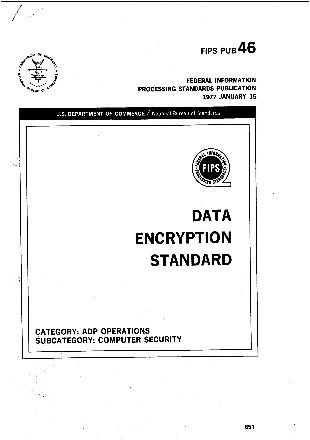
\includegraphics[width=0.85\textwidth]{../../images/python/page_004_img_01.jpeg}

\end{document}
